
\section{Focus surface stability checks}
\label{ap:focus_surfaces}

We test the stability of the NIKA2 focus surfaces, as obtained in
Sect.~\ref{sec:focus_surfaces}, against observation dates and
atmospheric conditions. We compare the focus surface obtained from the
five individual focus sequences used in Sect.~\ref{sec:focus_surfaces}.

In Figs.~\ref{fig:focus-stability-H}-\ref{fig:focus-stability-V}, we compare
the defocus along two perpendicular diameters across the
FOV. Although any direction would have been equivalent for this test, we choose to
position the diameters along-with and perpendicular-to the KID geometrical
grid to avoid the scatter due to KID non-alignement in any other
direction. The scatter is further mitigated by considering
four-detector-wide diameters as shown in upper the left corner of
Figs.~\ref{fig:focus-stability-H}-\ref{fig:focus-stability-V}.

The individual focus surfaces are in agreement with each other within
statistical errors. No systematics are observed depending on the
observation dates nor the atmospheric conditions. This indicates the
robustness of the focus surface estimates reported in
Sect.~\ref{sec:focus_surfaces}.




\begin{figure}
  %\begin{center}
  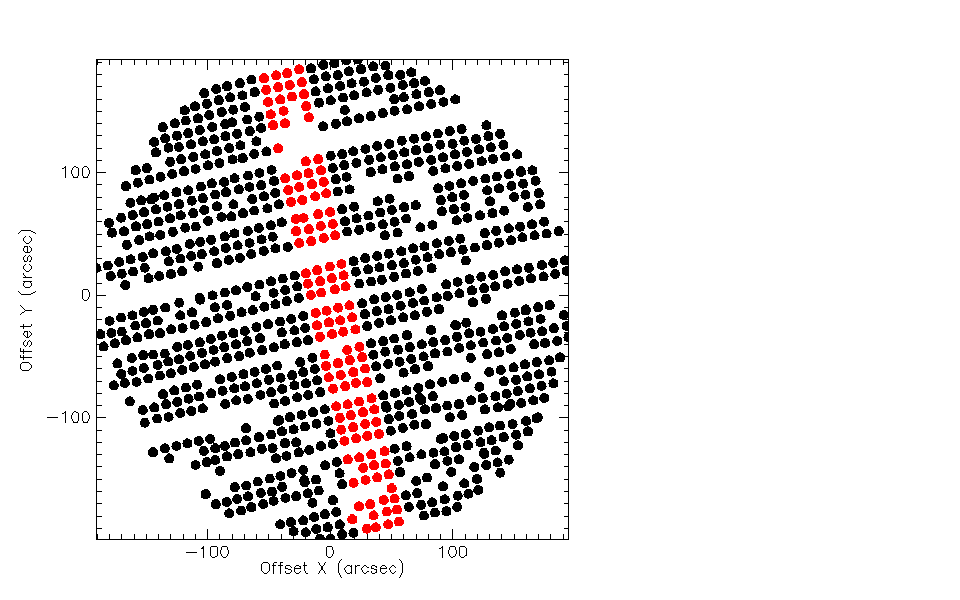
\includegraphics[trim={-2cm, 2cm, 0, 2cm}, clip, angle=0, scale=0.1]{Figures/fov_focus_stability_check_D1.png}
  \begin{center}
    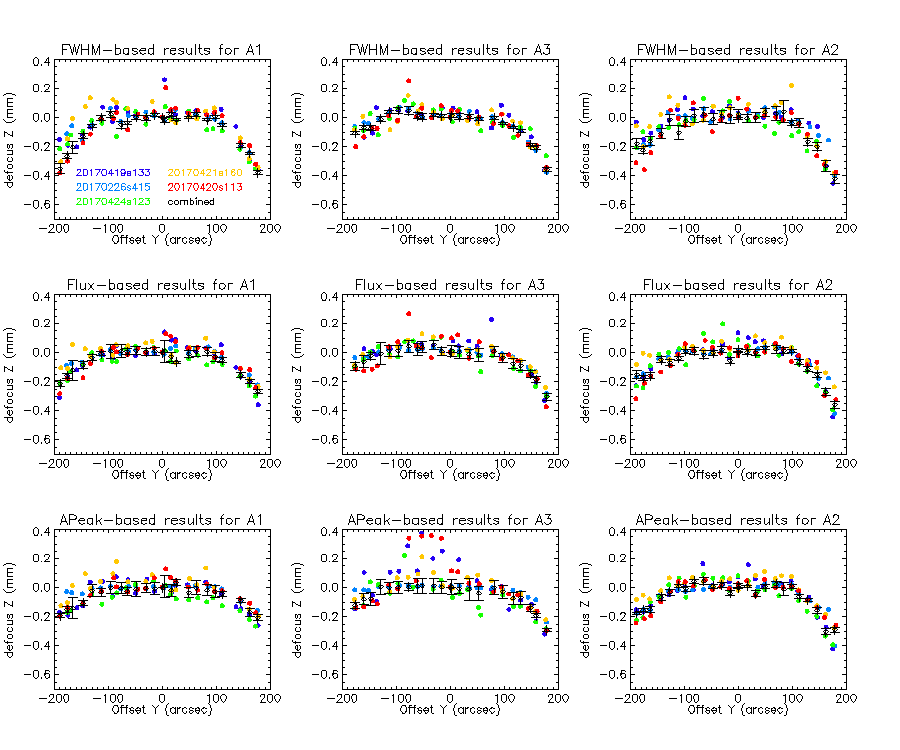
\includegraphics[trim={0, 1cm, 0, 1cm}, clip, angle=0, scale=0.45]{Figures/fov_focus_1D_Vband_5.png}
  \end{center}
  \caption[Stability of the focus surface across the sequences]{This
    series of plot show the relative focus with respect to the center
    (defocus) along the 'vertical diameter', that is a band of
    four-detector width across the FOV, which is vertical with respect to
    the detector geometrical grid, as illustrated by the plot in the
    upper left corner. The datapoints show the defocus along the
    'vertical diameter' estimated from the five focus sequences,
    namely $20170226s415\mbox{--}419$ (sky blue),
    $20170419s133\mbox{--}137$ (dark blue), $20170420s113\mbox{--}117$ (red),
    $20170421s160\mbox{--}164$ (yellow) and $20170424s123\mbox{--}127$
    (green), using the $z^{(a)}|_{\rm{fwhm}}$, $z^{(a)}|_{\rm{flux}}$ and
    $z^{(a)}|_{\rm{peak}}$ estimators from top to bottom, and for A1, A3 and
    A2 arrays from left to right. The black datapoints are the five-sequence combined defocus, as
    presented in Fig.~\ref{fig:focus-surfaces}, taken along the
    'vertical diameter', and the errorbars, the
    five-sequence combined defocus errors along the 'vertical
    diameter'.}
\label{fig:focus-stability-H}
\end{figure}


\begin{figure}
  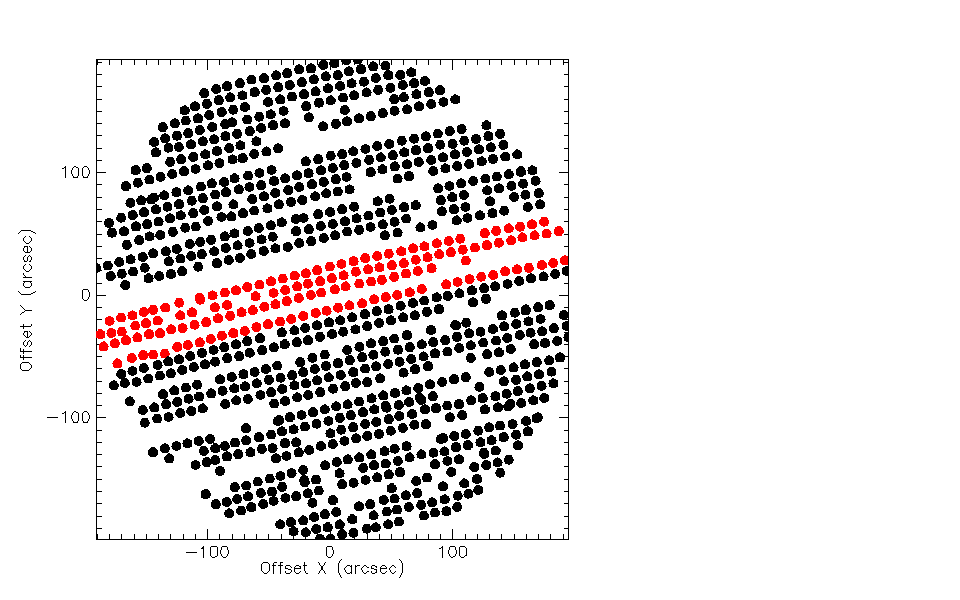
\includegraphics[trim={-2cm, 2cm, 0, 2cm}, clip, angle=0, scale=0.1]{Figures/fov_focus_stability_check_D2.png}
  \begin{center}
  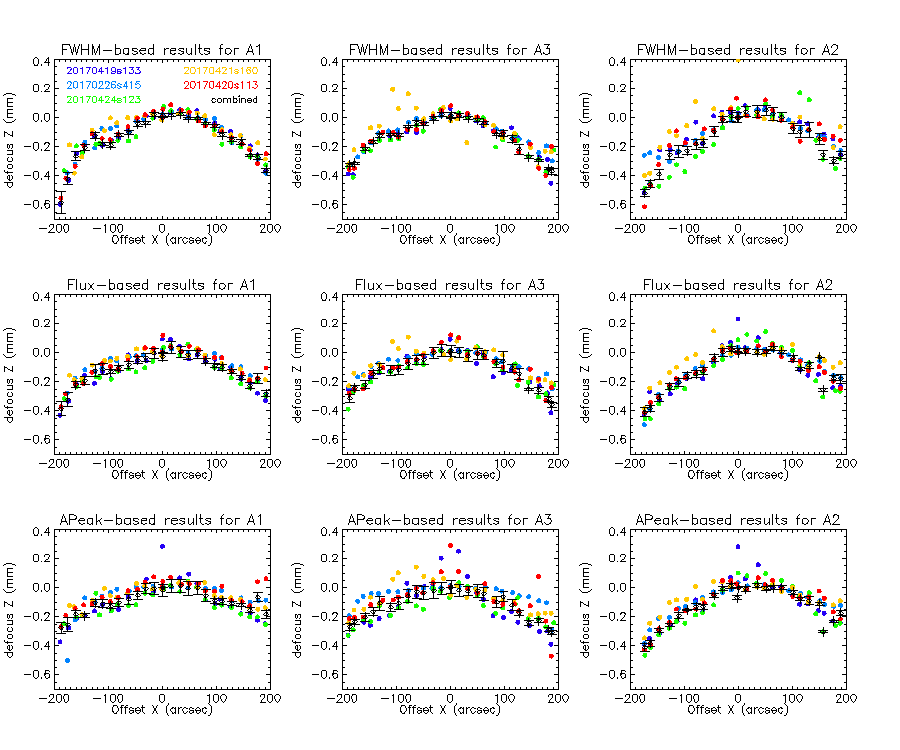
\includegraphics[trim={0, 1cm, 0, 1cm},clip, angle=0, scale=0.45]{Figures/fov_focus_1D_Hband_5.png}
  \caption[Stability of the focus surface across the sequences]{Same
    legend as in Fig.~\ref{fig:focus-stability-H}, but for the
    detectors located in an 'horizontal diameter', i.e. a band of
    four-detector width across the FOV, which is horizontal with respect to
    the detector geometrical grid, as illustrated by the plot in the
    upper left corner. }
\label{fig:focus-stability-V}
\end{center}
\end{figure}


